\documentclass{article}
\usepackage{graphicx} % Required for inserting images
\usepackage{float} % Required for controlling the position of images
\usepackage{listings} % Required for inserting code

\title{Assignment 4 - DD2424 - Vanilla RNN}
\author{Tristan Perrot}
\date{April 2024}


\begin{document}

\maketitle
\begin{center}
    
\includegraphics[scale=0.25]{images/KTH_logo_RGB_svart.png}
\end{center}

\section*{Gradient check}

After implementing forward pass and backward pass, I've checked the gradient computation by using the \texttt{autograd.grad} method of PyTorch. I've compared the gradients with the ones analytically computed and they were very close. The relative error was less than $10^{-7}$ for all the parameters:
\begin{verbatim}
Relative error on V: 3.21092130661782e-08
Relative error on c: 2.154427392042635e-08
Relative error on W: 4.962705801858647e-08
Relative error on b: 4.1212210533103644e-08
Relative error on U: 3.4753277589061327e-08
\end{verbatim}
These results show that the gradients are correctly computed.

\section*{Training}

\subsection*{Loss evolution}

After that, I trained the RNN for 10 epochs with \texttt{m=100, seq\_length=25, eta=.001, gamma=.9} as hyperparameters. The smooth loss evolution is shown in the following figure:

\begin{figure}[H]
    \centering
    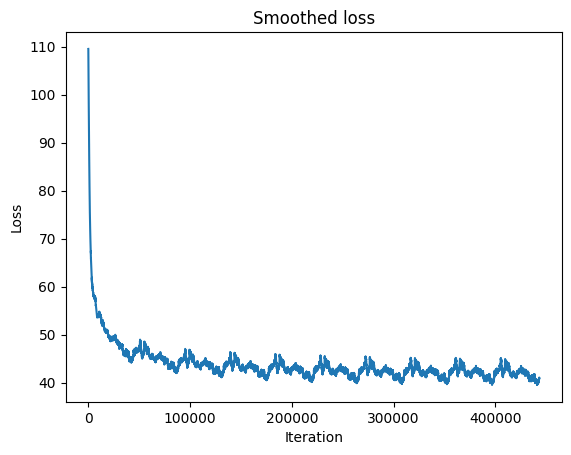
\includegraphics[width=\linewidth]{Result_Pics/loss.png}
    \caption{Smooth loss evolution for 10 epochs. The best loss observed was \textbf{39.5457}.}
\end{figure}

\subsection*{Synthesized text}

During the training, I've also generated some text using the RNN. The text is 200 characters long and generated before the first and every 10000 iterations of the first 1000000 iterations. Here is the evolution of the generated text:

\noindent \newline \textbf{Training - Iteration 0}
\begin{verbatim}[breaklines=true]
    gZQa!MZo0,S4Qi vPYyu•"z,.jgv9c:zFe6.mH
    dh4bqn	xMcH	xT:;VhrN/q-ozq!}COIDF4I2r1Fsz :LZn4M
    6I(gTdrGID4Qj!Xc!sT•j 	^,_DBxLQnrCVp.dG3deyehnwQ;
    FRmare(mbb6we/BEM
    'P1IxXcRu;B!Jx,'.üY!ic_ NpdR•N4y'gycNX17C1'U
\end{verbatim}
\textbf{Training - Iteration 10000 - Loss 53.84928512573242}
\begin{lstlisting}[breaklines=true]
    youndid , "cad ?"
    "
    ?ver.
    "I gat tum them an moca pat jasa ket see stica beront toly.
    "yary ak tharHe watf th ot't e's ilferly a mack oa miks at wh. Mr.
    "Cs tuplle wormartcrofn then mach, enstp easte
\end{lstlisting}
\textbf{Training - Iteration 20000 - Loss 49.59050369262695}
\begin{lstlisting}[breaklines=true]
    p an what ss d rim thag on of the laned lo y torer fimew bat rrecasking hid sitho, wnuch wnat hed a tired the "rme that itter coucan, dow ind into the the . He fire whout, in agelone, lyet upt mingete
\end{lstlisting}
\textbf{Training - Iteration 30000 - Loss 47.87261199951172}
\begin{lstlisting}[breaklines=true]
    ho, rest a bely.
    Harry featt Harry alllyand him, bobed every stire and a cleeped for there and grotes waswh therd were was galt 'eesarowly saring ghimming theme busicastef of -"
    inching .vin shis he h
\end{lstlisting}
\textbf{Training - Iteration 40000 - Loss 45.59083557128906}
\begin{lstlisting}[breaklines=true]
    hen comom nopidd they coldemort moodperburen, that eeding tion futa rish a folder whion finging faling reaning the ldeed if onesmid, thrihig an this froe.  e ffach as Harrys . . he oongw os thrteat gl
\end{lstlisting}
\textbf{Training - Iteration 50000 - Loss 47.49644470214844}
\begin{lstlisting}[breaklines=true]
    giwe thead and as the sofire.  alleras,"  now at them.
    "and iotrebin.  't  ibet hovee't and they have of aup, it to staarly that stoop who sarp ondem o
    "m,arssty ta the
    " maist you calks refecs breide
\end{lstlisting}
\textbf{Training - Iteration 60000 - Loss 45.70494842529297}
\begin{lstlisting}[breaklines=true]
    ry had mont the enturnicted the simest a said pirt of the groothing luch an the drey reattore from that theehel,  eeen the greaking crosten.

    Hest thought curtllehind pifiuct as their from whistentena
\end{lstlisting}
\textbf{Training - Iteration 70000 - Loss 45.728790283203125}
\begin{lstlisting}[breaklines=true]
    are you heflince he he's got and didn't a sive work. ". " gim, sairssair us and endcyouse fico, and whse put have clossarts factly and  wentferseing cheare foiner stuw handboing this you, the snorng i
\end{lstlisting}
\textbf{Training - Iteration 80000 - Loss 43.62993621826172}
\begin{lstlisting}[breaklines=true]
    weard now whowe out is youleor," said Harry lookedbeed aly. undle, umbeed.  encure aroom.  vell," gasilt.  re's ground.  Hagelys up.  said, along, you padned a bentn emcherrooked, The couiches.  eave
\end{lstlisting}
\textbf{Training - Iteration 90000 - Loss 44.04008483886719}
\begin{lstlisting}[breaklines=true]
    f fther to at head Harryones bellow, at thoys bey ask 's. ttlonmed mip, scroust studen, in theo Hagrick at him withort be and and the ent recet with his bark thabghtkwen, and lippith straking audiser
\end{lstlisting}
\textbf{Training - Iteration 100000 - Loss 45.647220611572266}
\begin{lstlisting}[breaklines=true]
    ituf langily as indotionaully. ."  eled down the ot diom.  "Hogwarts hood. . is a inky and returif down to choy, wh the befteIt who "andyou and "hbo the covllewtolpaling her anun, "nthints.  evary fur
\end{lstlisting}

\subsection*{Final synthesized text}

Then, with the best parameters, I've generated a text of 1000 characters. Here is the result:
\begin{lstlisting}[breaklines=true]
e into the ground, and  uiry his well, trymbled beath and Who saided them hag withail a please enease wolked yourmoned into Horut. ovither were hatched . ... we look.  His eyes rovane, how his eveningacketyns, still beay from the porion He that holding me . . . went ."  wadove bean befant .  adong to wailedy will.  He witch it.  I couck downed.  Harry to besher werry if he was rempalling me. , had about on read and that to he would him.  re indemation.  ye a drowing  Iat nlight the poonlytroy, at Dumbledore me shoon.  "I kninged, percmaster."
Harry teath Harry, and benafing the hat 
"b.  would he feight me.  "its at your's och to deSt you winnet this face ragged," said Dumbledore, he acondive.  as theel time . . . me bedork, thince.  on to him, stairIn right on but what he was will loiddre wandelf and bey" she was doing at the rectioc not, leggs as it.  Harry.
"" wiHa wiely in a dow a lined and chasice now along whelessinged them he teunded eps and think you gous, he plowered chsend be
\end{lstlisting}

\section*{Conclusion}

The RNN seems to be working well. The loss is decreasing during the training and the generated text is coherent. However, the text is not perfect and some words are not correctly spelled. The model could be improved by using Adam, word embeddings, or a more complex architecture like LSTM or GRU.

\end{document}